\documentclass{article}
\usepackage[english]{babel}
\usepackage{natbib}
\usepackage{anysize}
\marginsize{3cm}{3cm}{3cm}{3cm}
\usepackage{amsfonts,amsmath,amssymb,amsthm,bbm}
\usepackage{graphicx} 
%\usepackage{bmpsize}
\usepackage{color}
\usepackage{subfigure}
%usepackage[colorlinks=True, citecolor=blue]{hyperref}
%\usepackage{amssymb,amsthm,amsmath,bbm}
%\usepackage{mathrsfs}

\theoremstyle{plain}
\newtheorem{prop}{Proposition}
\theoremstyle{remark}
\newtheorem{rk}{Remark}

\def\beq{\begin{equation}}
\def\eeq{\end{equation}}
\def\fomega{\xi}
\def\cS{\mathcal{S}}
\def\cF{\mathcal{F}}
\newcommand{\IND}{\ensuremath{\mathbbm{1}}}
\def\figdir{figures}
\def\twofig{.48\textwidth}
\def\threefig{.32\textwidth}
\def\bom{{\boldsymbol{\fomega}}}
\def\sym{\text{sym}}
\def\XXX{\textcolor{red}{XXX}}
\def\th{\text{th}}
\def\textdots{\text{...}}
\title{On the zeros of the spectrogram of
  white noise}
\correspondingauthor{Samuel N. Quinn}
\email{squinn@cfa.harvard.edu}

\author[0000-0002-8964-8377]{Samuel N. Quinn}
\affiliation{\cfa}

\author[0000-0003-3182-5569]{Saul Rappaport}
\affiliation{\MIT}

\author[0000-0001-7246-5438]{Andrew Vanderburg}
\affiliation{\wisconsin}

\author[0000-0003-3773-5142]{Jason D. Eastman}
\affiliation{\cfa}

\author[0000-0002-6916-8130]{Lorne A. Nelson}
\affiliation{\bishops}

\author[0000-0003-3988-3245]{Thomas L. Jacobs}
\amateur
\affiliation{12812 SE 69th Place Bellevue, WA 98006, USA}

\author[0000-0002-8527-2114]{Daryll M. LaCourse}
\amateur
\affiliation{7507 52nd Place NE Marysville, WA 98270, USA}

\author{Allan R. Schmitt}
\amateur
\affiliation{616 W. 53rd. St., Apt. 101, Minneapolis, MN 55419, USA}

\author{Perry Berlind} 
\affiliation{\cfa}

\author[0000-0002-2830-5661]{Michael L. Calkins} 
\affiliation{\cfa}

\author[0000-0002-9789-5474]{Gilbert A. Esquerdo} 
\affiliation{\cfa}

\author[0000-0001-8638-0320]{Andrew W. Howard}
\affiliation{\caltech}

\author[0000-0002-0531-1073]{Howard Isaacson}
\affiliation{\berkeley}

\author[0000-0001-9911-7388]{David W. Latham}
\affiliation{\cfa}

% \author{others?}
% \noaffiliation{}

\date{}

\begin{document}
\maketitle
\begin{abstract}
In a recent paper, \cite{Fla15} has proposed filtering based on the zeros of a
spectrogram, using the short-time Fourier transform and a Gaussian window. His
results are based on empirical observations on the distribution of the zeros of
the spectrogram of white noise. These zeros tend to be uniformly spread over the
time-frequency plane, and not to clutter. Our contributions are threefold:
we rigorously define the zeros of the spectrogram of continuous white noise, we
explicitly characterize their statistical distribution, and we investigate the
computational and statistical underpinnings of the practical implementation of
signal detection based on the statistics of spectrogram zeros. In
particular, we stress that the zeros of spectrograms of white Gaussian noise
correspond to zeros of Gaussian analytic functions, a topic of recent
independent mathematical interest \citep{HKPV09}.
\end{abstract}

\section{Introduction}
\label{s:intro}
Spectrograms are a cornerstone of time-frequency analysis \citep{Fla98}. They are quadratic time-frequency representations of a
signal \cite[Chapter 4]{Gro01}, associating to each time and frequency a real
number that measures the energy content of a signal at that time and frequency, unlike global-in-time tools such as the Fourier
transform. Since it is natural to expect that there is more energy where there
is more information or signal, most methodologies have focused on detecting and
processing the local maxima of the spectrogram \citep{Coh95, Fla98, Gro01}. Usual techniques include \emph{ridge extraction},
e.g., to identify chirps, or \emph{reassignment} and \emph{synchrosqueezing}, to
better localize the maxima of the spectrogram before further quantitative
analysis. 

In contrast, \cite{Fla15} has recently observed that the locations of the zeros of a
spectrogram in the time-frequency plane almost completely characterize the
spectrogram, and he proposed to use the point pattern formed by the zeros in
filtering and reconstruction of signals in noise. This proposition stems from
the empirical observation that the zeros of the short-time Fourier transform of
white noise are uniformly spread over the time-frequency plane, and tend not to
clutter, as if they repelled each other. In the presence of a signal, zeros are
absent in the time-frequency support of the signal, thus creating large holes
that appear to be very rare when observing pure white noise. This leads to testing
the presence of signal by looking at statistics of the point pattern of zeros,
and trying to identify holes. In this paper, we attempt a formalization of the
approach of \cite{Fla15}. To this purpose, we put together notions of signal
processing, complex analysis, probability, and spatial statistics.

Our contributions are threefold: we rigorously define the zeros of the
spectrogram of continuous white noise, we explicitely characterize their
statistical distribution, and we investigate the computational and statistical
underpinnings of the practical implementation of signal detection. In
particular, we stress that zeros of spectrograms of white noise correspond to
zeros of Gaussian analytic functions, a topic of recent independent mathematical interest \citep{HKPV09}.

In short, our approach starts from the usual definition of white noise as a random
tempered distribution. Using a classical equivalence between the short-time
Fourier transform and the Bargmann transform, we show that the short-time
Fourier transform of white noise can be identified with a random analytic
function, so that we can give a precise meaning to the zeros of the spectrogram of white
noise. It turns out that real and complex Gaussian white noises lead to
recently studied random analytic functions, with completely characterized zeros. We
then investigate how to leverage probabilistic information on these zeros to design
statistical detection procedures. This includes linking probability and
complex analysis results to the discrete implementation of the Fourier
transform.

The rest of the paper is organized as follows. In Section~\ref{s:preliminary},
we introduce the relevant notions of complex analysis, probability, and spatial
statistics. In Section~\ref{s:real}, we characterize the zeros of the short-time
Fourier transform of real white noise, while the complex and the analytical case
are treated in Section~\ref{s:complex}. In Section~\ref{s:stats}, we investigate
the relation between the previous sections and the usual discrete implementation
of the Fourier transform, and we demonstrate a detection task using the spectrogram zeros.


\section{Spectrograms, complex analysis, and point processes}
\label{s:preliminary}
%\vspace{-1em}
\section{Preliminaries}
%\vspace{-1em}
\label{sec:preliminaries}
Datasets $X, X' \in \mathcal{X}$ are neighbors if they differ by no more than one datapoint -- i.e., $X \simeq X'$ if $d(X, X') \leq 1$. We will define $d(\cdot)$ to be the number of coordinates that differ between two datasets of the same size $n$: $d(X, Y) = \#\{i \in [n]: X_i \neq Y_i  \}$.

We use $||\cdot||$ to denote the radius of the smallest Euclidean ball that contains the input set, e.g. $||\mathcal{X}|| = \sup_{x \in \mathcal{X}} ||x||$.

The parameter $\phi$ denotes the privacy parameters associated with a mechanism (e.g. noise level, regularization). $\mathcal{M}_{\phi}$ is a mechanism parameterized by $\phi$.
For mechanisms with continuous output space, we will take $\text{Pr}[\mathcal{M}(X) = y]$ to be the probability density function of $\mathcal{M}(X)$ at $y$.



    \begin{definition}[Differential privacy \citep{dwork2006calibrating}] \label{def:dp}
        Fix $\epsilon, \delta \geq 0$. 
A randomized algorithm $\mathcal{M}: \mathcal{X} \rightarrow \mathcal{S}$ satisfies $(\epsilon, \delta)$-DP if for all neighboring datasets $X \simeq X'$ and for all measurable sets $S \subset \mathcal{S}$, 
            \[\text{Pr}\big[\mathcal{M}(X) \in S\big] \leq e^{\epsilon}\text{Pr}\big[\mathcal{M}(X') \in S\big] + \delta.\]
    \end{definition}
%\vspace{-3mm}
% We now define \emph{data-dependent} differential privacy that conditions on an input dataset $X$. 

% \begin{definition}[Data-dependent privacy\cite{papernot2018scalable}]\vspace{-1mm}
% \label{def:data_dep_dp}
% Suppose we have $\delta > 0$ and a function $\epsilon: \mathcal{X} \rightarrow \mathbb{R}$. We say that mechanism $\mathcal{M}$ satisfies ($\epsilon(X), \delta$) data-dependent DP for dataset $X$ if for all possible output sets $S$ and neighboring datasets $X'$,
% \begin{align*}
%     \text{Pr}\big[\mathcal{M}(X) \in S\big] &\leq e^{\epsilon(X)}\text{Pr}\big[\mathcal{M}(X') \in S\big] + \delta, \\
%       \text{Pr}\big[\mathcal{M}(X') \in S\big] &\leq e^{\epsilon(X)}\text{Pr}\big[\mathcal{M}(X) \in S\big] + \delta.
% \end{align*}
% \end{definition}

%\subsection{Additive Noise Mechanisms}
Suppose we wish to privately release the output of a real-valued function $f: \mathcal{X} \rightarrow \mathcal{R}$. We can do so by calculating the \emph{global sensitivity} $\Delta_{GS}$, calibrating the noise scale to the global sensitivity and then adding sampled noise to the output.



\begin{definition}[Local / Global sensitivity]
The local $\ell_*$-sensitivity of a function $f$ is defined as $\Delta_{LS}(X) = \max\limits_{X \simeq X'} || f(X) - f(X') ||_* $ and the global sensitivity of $f$ is $\Delta_{GS} = \sup_X \Delta_{LS}(X)$.
% The local $\ell_*$-sensitivity of a function $f: \cX \to \mathbb{R}^d$ is defined as $\Delta_{LS}(X) = \max\limits_{X \simeq X'} || f(X) - f(X') ||_* $ and the global sensitivity of $f$ is $\Delta_{GS} = \sup_X \Delta_{LS}(X)$.
\end{definition}
%\vspace{-2mm}
% The choice of $\ell_*$ depends on which kind of noise we use, e.g., $\ell_2$-norm is used for Gaussian noise.

\begin{comment}

\begin{definition}[Global sensitivity]
The global $\ell_*$-sensitivity of a function $f: \mathcal{X} \rightarrow \mathcal{R}^d$ is defined as
\begin{align*}
    \Delta_{GS} &= \max\limits_{X, X' \in \mathcal{X}:X \simeq X'} || f(X) - f(X') ||_*. 
\end{align*}
\end{definition}
\begin{definition}[Laplace mechanism]
The Laplace mechanism $\mathcal{M}: \mathcal{X} \rightarrow \mathbb{R}$ applied to a function $f$ is given as
\begin{align*}
    \mathcal{M}(X) &= f(X) + \text{Lap}\left(b \right).
\end{align*}
\end{definition}
\begin{theorem}
Suppose the function $f: \mathcal{X} \rightarrow \mathbb{R}$ has global $\ell_1$-sensitivity $\Delta_f$. Then the Laplace mechanism satisfies $\epsilon$-differential privacy with noise parameter $b = \Delta_f/\epsilon$.	 \vspace{-2mm}
\end{theorem}

\begin{definition}[Gaussian mechanism]
The Gaussian mechanism $\mathcal{M}: \mathcal{X} \rightarrow \mathbb{R}$ applied to a function $f$ is given as
\begin{align*}
    \mathcal{M}(X) &= f(X) + \mathcal{N}(0, \sigma^2).
\end{align*}
\end{definition}
\begin{theorem}
Suppose the function $f: \mathcal{X} \rightarrow \mathbb{R}$ has global $\ell_2$-sensitivity $\Delta_f$. Then the Gaussian mechanism satisfies $(\epsilon, \delta)$-differential privacy with noise parameter $\sigma = \Delta_f\sqrt{2 \log(1.25/\delta)}/\epsilon$.
\end{theorem}
Both the Laplace and Gaussian mechanisms generalize easily to releasing the output of a $d$-dimensional function $f$ by adding i.i.d. noise to each coordinate.
\begin{definition}[Local sensitivity]
The local $\ell_*$-sensitivity of a function $f: \mathcal{X} \rightarrow \mathbb{R}^d$ is defined as
\begin{align*}
    \Delta_{LS}(X) &= \max\limits_{X \simeq X'} || f(X) - f(X') ||_*. 
\end{align*}
\end{definition}
\end{comment}
% \todo{Define Global sensitivity}
%define global/local sensitivity
%Laplace, Gaussian mech
% explain how related to PTR and its generalization

%\vspace{-0.em}
\subsection{Propose-Test-Release}
%\vspace{-0.5em}
Calibrating the noise level to the local sensitivity $\Delta_{LS}(X)$ of a function would allow us to add less noise and therefore achieve higher utility for releasing private queries. However, the local sensitivity is a data-dependent function and na\"ively calibrating the noise level to $\Delta_{LS}(X)$ will not satisfy DP.

PTR resolves this issue in a three-step procedure: \textbf{propose} a bound on the local sensitivity, privately \textbf{test} that the bound is valid (with high probability), and if so calibrate noise according to the bound and \textbf{release} the output.

% \begin{figure}[t]
% \vspace{-1em}
% \centering
% \resizebox{0.95\columnwidth}{!}{%
% \begin{minipage}{0.50\textwidth}
% \begin{algorithm}[H]
% \caption{Propose-Test-Release \cite{dwork2009differential}}
% \label{alg:classic_ptr}
% \begin{algorithmic}[1]
% \STATE{\textbf{Input}: Dataset $X$; privacy parameters $\epsilon,\delta$; proposed bound $\beta$ on $\Delta_{LS}(X)$; query function $f: \mathcal{X} \rightarrow \mathbb{R}$.}
% \STATE{\textbf{Output}: $f^P(X)$ or $\perp$.}
% \STATE{Compute the distance $\gamma(X)$ to the nearest dataset $X''$ such that $ \Delta_{LS}(X'')> \beta$:
% $\gamma(X) = \min\limits_{X''} \{ \text{dist}(X, X''): \Delta_{LS}(X'')> \beta \}$.}
% \STATE{Privately release $\gamma^P(X) = \gamma(X) + \text{Lap}\left(\frac{1}{\epsilon}\right)$.}
% \IF{$\gamma^P(X) > \dfrac{\log(1/\delta)}{\epsilon}$}\vspace{-1pt}
% \STATE{Release $f^P(X) = f(X) + \text{Lap}\left(\frac{\beta}{\epsilon}\right)$.}\vspace{-2pt}
% \ELSE
% \STATE{Output $\perp$.}\vspace{-1pt}
% \ENDIF
% \end{algorithmic}
% \end{algorithm}
% \end{minipage}
% \quad
% \begin{minipage}{0.46\textwidth}
% \begin{algorithm}[H]
% \caption{Generalized PTR}
% \label{alg:gen_ptr}
% \begin{algorithmic}[1]
% \STATE{{Input}: Proposed~parameter~$\phi$;~privacy~parameters~$\epsilon,  \hat{\epsilon}, \hat{\delta}$; dataset $X$;\blue{an $(\epsilon,\delta)$~DP test $\cT$; ~data-dependent~DP~function~$\epsilon_{\phi}(\cdot, \hat{\delta})$;~mechanism~$\mathcal{M}_{\phi}$.}}
% \STATE{\textbf{Output}: 
% $\mathcal{M}_{\phi}(X)$ or $\perp$.}
% \STATE{Let $\cT$ privately test if $\epsilon_\phi(X,\hat{\delta}) \leq \hat{\epsilon}$.}% with privacy limit $(\hat{\epsilon}, \hat{\delta})$ }.
% \IF{the test $\cT$ passes}
% \vspace{1pt}
% \STATE{Run $\theta = \mathcal{M}_{\phi}(X)$ and output $\theta$.}\vspace{2pt}

% \ELSE \vspace{2pt}

% \STATE{Output $\perp$.}\vspace{2pt}

% \ENDIF
% \end{algorithmic}
% \end{algorithm}
% \end{minipage}
% }
% \vspace{-1em}
% \end{figure}


% \begin{theorem} 
% Algorithm~\ref{alg:classic_ptr} satisfies ($2 \epsilon, \delta$)-DP.
% \cite{dwork2009differential}
% \end{theorem}

PTR privately computes the distance $\cD_{\beta}(X)$ between the input dataset $X$ and the nearest dataset $X''$ whose local sensitivity exceeds the proposed bound $\beta$:
\begin{align*}
    \cD_{\beta}(X) = \min\limits_{X''} \{ d(X, X''): \Delta_{LS}(X'')> \beta \}.
\end{align*}
%\vspace{-.8em}
% The $\epsilon$-DP "test" fails (with probability $\delta$) if PTR decides to release $f^P(X)$ when $\gamma(X) = 0$, i.e. when dataset $X$ has local sensitivity greater than $\beta$.

\begin{figure}[H]
\vspace{-1.4em}
\centering
% \resizebox{0.95\columnwidth}{!}{%
% \begin{minipage}{0.54\textwidth}
\begin{algorithm}[H]
\caption{Propose-Test-Release \citep{dwork2009differential}}
\label{alg:classic_ptr}
\begin{algorithmic}[1]
\STATE{\textbf{Input}: Dataset $X$; privacy parameters $\epsilon,\delta$; proposed bound $\beta$ on $\Delta_{LS}(X)$; query function $f: \mathcal{X} \rightarrow \mathbb{R}$.}
% \STATE{\textbf{Output}: $f^P(X)$ or $\perp$.}
% \STATE{Compute the distance $\gamma(X)$ to the nearest dataset $X''$ such that $ \Delta_{LS}(X'')> \beta$.}
% \STATE{Privately release $\gamma^P = \gamma(X; \beta) + \text{Lap}\left(\frac{1}{\epsilon}\right)$.}

\STATE{\textbf{if} $\cD_{\beta}(X) + \text{Lap}\left(\frac{1}{\epsilon}\right) \leq \frac{\log(1/\delta)}{\epsilon}$ \textbf{then} output $\perp$,}
\STATE{\textbf{else} release $f(X) + \text{Lap}\left(\frac{\beta}{\epsilon}\right)$.}
\end{algorithmic}
\end{algorithm}
\end{figure}
%\vspace{-.8em}
\begin{theorem} 
Algorithm~\ref{alg:classic_ptr} satisfies ($2 \epsilon, \delta$)-DP.
\citep{dwork2009differential}
\end{theorem}
%\vspace{-1em}
Rather than proposing an arbitrary threshold $\beta$, one can also privately release an upper bound of the local sensitivity and calibrate noise according to this upper bound. This was used for node DP in graph statistics \citep{kasiviswanathan2013analyzing}, and for fitting topic models using spectral methods \citep{decarolis2020end}.

%This gives a more efficient alternative and avoids the need to propose $\beta$. This variant is  the local sensitivity itself has a global sensitivity.

%there exist other variants of PTR --- e.g., compute a differentially private upper bound of the local sensitivity and calibrate noise according to this upper bound. This type of PTR requires a global sensitivity of the local sensitivity. We refer readers to the excellent summary of PTR in  section 3 of \citet{vadhan2017complexity}.

% We may mention other types of PTR: propose and release
% There are other variants of PTR... 
% \vspace{-1mm}
% \subsection{Motivation}
% \vspace{-1mm}
% Why do we want to generalize PTR beyond noise-adding mechanisms? For other mechanisms, the local sensitivity either does not exist or is only defined for specific data-dependent quantities (e.g., the sensitivity of the score function in the exponential mechanism) rather than the mechanism's output. We give a concrete example below. 

%In this section, we give a concrete example to demonstrate this limitation and motivate our generalization.
%This section discusses a few limitations of PTR approaches that motivated our work.
%Let us first ask, ``is PTR a general framework applicable to any mechanism with a data-dependent analysis?'' If so, we could explore other less costly approaches to privately test the local sensitivity.

%However, the answer is unfortunately ``no''.  The reasons are twofold. First, the framework above applies only to ``noise-adding'' mechanisms --- where we have a well-defined local sensitivity (of the output), and the noise scale is calibrated according to that. For other non-noise-adding mechanisms, the local sensitivity either does not exist or is only defined for specific data-dependent quantities (e.g., the sensitivity of the score function in the exponential mechanism) rather than the mechanism's output. Consider the difficulties of applying PTR to the following example.


% \begin{example}[Private posterior sampling]\label{exp: posterior}
% Let $\cM: \cX\times \cY \to \Theta $ be a private posterior sampling   mechanism~\citep{minami2016differential,wang2015privacy,gopi2022private} for approximately minimizing $F_{X}(\theta)$. % for linear regression problem, i.e., $\min_{\theta} \frac{1}{2}||y-X\theta||^2 + \lambda ||\theta||^2$. 
% $\cM$ samples $\theta \sim P(\theta)\propto e^{-\gamma(F_X(\theta)+ 0.5\lambda ||\theta||^2)}$ with parameters $\gamma, \lambda$. $\gamma,\lambda$ cannot be appropriately chosen for this mechanism to satisfy DP without going through a sensitivity calculation of $\arg\min F_X(\theta)$. In fact, the global and local sensitivity of the minimizer is unbounded even in linear regression problems, i.e., when $F_X(\theta) = \frac{1}{2}||y-X\theta||^2.$ 
% %The local sensitivity $\Delta:=||P_{X,y}(\theta)-P_{X', y'}(\theta)||$ is not well-defined  for the sampling algorithm, thus the standard PTR is not applicable.  
% \end{example}
% Output perturbation algorithms do work for the above problem when we regularize, but they are known to be suboptimal in theory and in practice \cite{chaudhuri2011differentially}.% do not achieve the level of utility in theory and in practice when comparing to posterior sampling. 
 

% Moreover, even in the cases of noise-adding mechanisms where PTR seems to be applicable, it does not lead to a tight privacy guarantee. Specifically, by an example of privacy amplification by post-processing (Example~\ref{exp: binary_vote} in the appendix), we demonstrate that the local sensitivity does not capture all sufficient statistics for data-dependent privacy analysis and thus is loose.

% Instead of identifying sufficient statistics of each mechanism, we develop a unified framework --- generalized PTR, offering the flexibility for any mechanism to exploit data-dependent quantities.

% \textbf{On data-dependent DP losses.} In addition to the above, there has been an increasing list of empirical DP work that fix the parameters of a randomized algorithm while reporting the resulting data-dependent DP losses $\epsilon(\text{Data})$ after running on a specific dataset \citep{ligett2017accuracy,papernot2018scalable,zhu2020private, feldman2021individual}. The data-dependent DP losses are often smaller than the worst-case DP losses, but technically speaking, these algorithms are not formally DP with DP guarantees any smaller than that of the worst-case. In addition, the data-dependent DP losses themselves are sensitive, and thus cannot be reported. A typical solution is to privately release $\epsilon(\text{Data})$, but it still does not satisfy DP as this would require a prescribed $(\epsilon,\delta)$-DP parameter to be satisfied for all input datasets. Part of our contribution is to resolve this conundrum by showing that a simple post-processing step of the privately released upper bound of $\epsilon(\text{Data})$ gives a formal DP algorithm.
%\yq{Shall we combine this part with the related work section?}

%Instead,  exploits data-dependent quantities by first privately choosing $\gamma, \lambda$ adapted to the dataset and then applying posterior sampling with the sanitized parameters.  


\section{The spectrogram of real white noise}
\label{s:real}
In this section, we define real white noise, and examine the zeros of its
spectrogram. 
\subsection{Definitions}

To define white noise, we closely follow \cite[Chapter 2.1]{HOUZ10} through a
classical approach that does not require defining Brownian motion first. We denote by $\cS=\cS(\mathbb{R})$
the Schwartz space of rapidly decaying smooth complex-valued functions of a real
variable. The dual $\cS'=\cS'(\mathbb{R})$, equipped with the weak-star
topology, is the space of \emph{tempered distributions}. The topology yields the
Borel sigma-algebra $\mathcal{B}(\cS')$ on $\cS'$. Now, the Bochner-Minlos
theorem \citep[Theorem 2.1.1]{HOUZ10} states that there exists a unique probability
measure $\mu_1$ on $(\cS',\mathcal{B}(\cS'))$ such that 
\beq
\forall \phi\in \cS, \quad \mathbb{E}_{\mu_1}e^{i\langle \cdot,\phi \rangle} =
e^{-\frac{1}{2}\Vert \phi\Vert_2^2}.
\label{e:bochner}
\eeq
We call this measure white noise, and $(\cS',B(\cS'),\mu_1)$ the white noise
probability space. In particular, \eqref{e:bochner}
implies that for a random variable\footnote{We use the term \emph{random variable}, but it is also customary to call $\fomega$ a \emph{generalized random process} in the literature.} with distribution
$\mu_1$ and a set of real-valued orthonormal functions $\varphi_1,\dots,\varphi_p$ in $\cS$, the vector
$(\langle \fomega_1,\varphi_1 \rangle,\dots,\langle \fomega_p,\varphi_p \rangle)$
follows a real multivariate Gaussian, with mean zero and identity covariance matrix,
see \cite[Lemma 2.1.2]{HOUZ10}. This is in accordance with the usual heuristic of white noise having a Dirac delta covariance function.

Let $\fomega$ be a random variable with distribution $\mu_1$.
If $g\in\cS$, then $(u,v)\mapsto M_v T_u g$ is in $\cS$, so that we can define
the STFT of $\fomega$ as the random function
$$ u,v\mapsto \langle \fomega,  M_v T_u g \rangle.$$
From now on, we restrict ourselves to the Gaussian window $g(x) =
2^{1/4}e^{-\pi x^2}$, normalized so that $\Vert g\Vert_2 = 1$. We are interested
in defining and studying the zeros of the spectrogram
\beq
\label{e:spectrogram}
S:u,v\mapsto \vert \langle \fomega,  M_v T_u g \rangle\vert^2.
\eeq

\subsection{Characterizing the zeros}
\label{e:zerosSymmetricGAF}
We work in two steps: in Proposition~\ref{p:series}, we identify each value
$S(u,v)$ in \eqref{e:spectrogram} as a limit in $L^2(\mu_1)$, and we then
show in Proposition~\ref{p:symmetricPlanarGAF} that the resulting random field
defines an entire function, the zeros of which are known.
\begin{prop}
Let $u,v\in\mathbb{R}^2$, and write $z=u+iv\in\mathbb{C}$. Then
\beq
\langle \fomega,  M_v T_u g \rangle = \sqrt{\pi} e^{i\pi uv}e^{-\frac{\pi}{2}\vert z\vert^2} \sum_{k=0}^{\infty}\langle \fomega,h_k
\rangle \frac{\pi^{k/2}z^k}{\sqrt{k!}} 
\label{e:series}
\eeq
where $(h_k)$ denote the orthonormal Hermite functions \cite[Section 2.2.1]{HOUZ10}, and convergence is in $L^2(\mu_1)$.
\label{p:series}
\end{prop}
\begin{rk}
\label{r:zeros}
Note that in Proposition~\ref{p:series}, $u$ and $v$ are fixed, and the equality
is a limit in $L^2(\mu_1)$. It is still too early to identify the zeros of
the left-hand side to the zeros of the right-hand side.
\end{rk}
\begin{rk}
Note that our choice of the window $g(x) = 2^{1/4}e^{-\pi x^2}$ is made to
simplify expressions. The proof of Proposition~\ref{p:series}, along with
Sections~\ref{s:hermite} and \ref{s:bargmann}, immediately yield that for a non-unit Gaussian window $g_a(x) \propto \exp(-\pi
a^2 x^2)$, Proposition~\ref{p:series} is unchanged, provided that $z$ is defined
as $z = au + iv/a$ and a constant is prepended to the RHS of
\eqref{e:series}. In other words, given a particular value of $a$, it is always possible to
dilate/squeeze the time-frequency axes to obtain the results detailed
here for $a = 1$. 
\end{rk}
\begin{proof}
Let $u,v\in\mathbb{R}^2$. Decomposing $M_v T_u g$ in the Hermite basis $(h_k)$ of
$L^2(\mathbb{R})$, it comes
\begin{eqnarray}
\langle \fomega, M_v T_u g \rangle &=& \sum_{k=0}^\infty \langle \fomega,h_k
  \rangle \langle  M_v T_u g,h_k\rangle\nonumber\\
&=&  \sum_{k=0}^\infty \langle \fomega,h_k
  \rangle \overline{V_g(h_k)(u,v)}
\label{e:decomp}
\end{eqnarray}
where the limits are in $L^2(\mu_1)$. The STFT of Hermite functions is
well-known, see e.g. the proof of \cite[Proposition 3.4.4]{Gro01} or our Section~\ref{s:bargmann}, and it reads
\beq 
V_g(h_k)(u,v) = e^{-i\pi
  uv}e^{-\frac{\pi}{2}(u^2+v^2)}\frac{\pi^{k/2}}{\sqrt{k!}}(u-iv)^k.
\label{e:HermiteSTFT}
\eeq
Plugging \eqref{e:HermiteSTFT} into \eqref{e:decomp} yields the result.
\end{proof}

Now we focus on the regularity of the right-hand side of \eqref{e:series}.
\begin{prop}
\label{p:symmetricPlanarGAF}
The random series
\beq
\label{e:symmetricPlanarGAF}
\sum_{k=0}^{\infty}\langle \fomega,h_k
\rangle \frac{\pi^{k/2}z^k}{\sqrt{k!}}
\eeq
$\mu_1$-almost surely defines an entire function. 
\end{prop}
\begin{proof}
By \cite[Lemma 2.1.2]{HOUZ10}, ($\langle \fomega,h_k
\rangle)_{k\geq 0}$ are i.i.d. unit real Gaussians. We then apply the first part
of \cite[Lemma 2.2.3]{HKPV09}.
\end{proof}
Since both $L^2$ and almost sure convergence imply convergence in probability,
$L^2$ and almost sure limits have to be the same. In particular,
Propositions~\ref{p:series} and \ref{p:symmetricPlanarGAF} together yield that the
distribution of the zeros of the spectrogram $S$ in \eqref{e:spectrogram} is
the same as the distribution of the zeros of the random entire function
\eqref{e:symmetricPlanarGAF}. This answers Remark~\ref{r:zeros}. In particular,
we now know that the zeros of $S$ are isolated.

The entire function in \eqref{e:symmetricPlanarGAF} is called the
\emph{symmetric planar Gaussian analytic function} (GAF), and a few of its properties are known
\citep{Fel13}. However, its zeros do not define a stationary point process. In
particular, a portion of the zeros concentrate on the real axis, see
Figure~\ref{f:symmetricPlanarGAF}. Intuitively, one can approximate the zeros of
\eqref{e:symmetricPlanarGAF} by the zeros of the random polynomial obtained from
truncating the series. The resulting polynomial has real coefficients, and it is
thus expected to have real zeros as well as pairs of conjugate complex zeros. As a side note, the number of real zeros is a
topic of study on its own, see e.g. \citep{ScMa08}. 

\begin{figure}
\subfigure[Real white noise/symmetric GAF]{
\includegraphics[width=\twofig]{\figdir/realWGNdist.pdf}
\label{f:symmetricPlanarGAF}
}
\subfigure[Complex white noise/planar GAF]{
\includegraphics[width=\twofig]{\figdir/complexWGN/complexWGNdist.pdf}
\label{f:complexPlanarGAF}
}
\caption{The spectrogram of (a) a realization of real white noise, and (b) a
  realization of complex white noise. The right and top plots on each panel show
marginal histograms, superimposed with the theoretical marginal density, see
text for details.}
\label{f:GAFs}
\end{figure}

Coming back to our problem of detecting signals, this non-stationarity
makes it uneasy to approach via traditional spatial statistics techniques, which
often assume some degree of stationarity. However, there is a stationary point
process that is a good approximation for the zeros of the symmetric planar GAF,
and that has been studied in depth. This point process is the zeros of the
\emph{planar GAF}, the entire function corresponding to the STFT of complex
white noise. 


\section{The case of complex white noise}
\label{s:complex}
\section{Existence and Complexity}\label{sec:complex}
In this section we discuss the computational issues surrounding the three types of $\theta$ fair flows. The existence of Pure Nash equilibrium in nonatomic routing games guarantees the existence of any $\theta$ fair flow for $\theta\geq 1$. The next question would be whether we can compute $\theta$ fair flows with good social cost.  In particular, we consider the following problems:
\begin{enumerate}
	\item[(P1)] Find a $\theta$-EF path flow with the minimal social cost.
	\item[(P2)] Find a $\theta$-UNE path flow with the minimal social cost.
	\item[(P3)] Find a $\theta$-PNE edge flow with the minimal social cost.
\end{enumerate}
We show that for large $\theta$, the socially optimal flow is guaranteed to be contained in those $\theta$-flows, and hence the optimal $\theta$-flows be computed efficiently.  However, for small $\theta$, we will show that solving Problem~(P1) and Problem~(P2) is NP-hard, while it remains open whether Problem~(P3) can be computed efficiently.  
More precisely, for a latency class $\mc{L}$, this particular threshold is $\gamma(\mc{L})= \min\{\gamma: \ell^{*}(x)\leq \gamma \ell(x), \forall \ell\in \mc{L}, \forall x\geq 0\}$, where $\ell^{*}(x)= \ell(x)+x\ell'(x)$.  The main result of this section is given as follows:
\begin{theorem}
	%\begin{enumerate}
	%\item \fin{
	For any multi commodity instance $\mc{G}$ 
	with latency functions in any class $\mc{L}$, there are polynomial time algorithms\footnotemark $\, $  for solving Problem~(P1)-(P3) 
	for $\theta \ge \gamma(\mc{L})$. %, for any class $\mc{L}$.
	%
	On the other hand, it is NP-hard to solve Problem~(P1) for $\theta \in [1, \gamma(\mc{L}))$ and Problem~(P2) for $\theta \in (1, \gamma(\mc{L}))$, for  arbitrary single commodity instances %$\mc{G}$ 
	with latency functions in an arbitrary class $\mc{L}$.
	%\end{enumerate}
	\label{thm:main_hardness}
\end{theorem} 

\footnotetext{The existence of polynomial time algorithms for our problem depends on the assumption that we can minimize separable convex functions with linear constraints in polynomial time; numerical issues for convex optimization are discussed in \cite{hochbaum1990convex,  nemirovski2004interior} and are beyond the scope of our work.}
%on the existence of polynomial time algorithms for minimizing separable convex functions with linear constraints upto arbitrary precision. See~\cite{hochbaum1990convex,  nemirovski2004interior}   for details, which are quite technical for the scope of this paper.}}





In the following sections, we first prove the first part of Theorem \ref{thm:main_hardness}. Right after we show that, for any $\theta$, from any $\theta$ fair flow we may get another $\theta$ fair flow, which uses only polynomially many paths. This, on the one hand, serves as a clarification that the difficulty of problems~(P1)-(P3) does not lie in the size of their solutions. On the other hand, it helps in showing that the decision version of these problems lies in NP, since for a YES instance, a non-deterministic machine will (non-deterministically) choose a path flow of polynomial size and in polynomial time check that it satisfies the conditions needed. Finally, the second part of Theorem \ref{thm:main_hardness} follows from an NP-hardness proof for a stronger version of the decision versions of problems~(P1) and (P2) (Theorem \ref{thm:12Hard}).


\subsection{When the Social Optimum is Guaranteed to be the Solution}\label{sec:complexity_so}
First, we show that Problems~(P1)-(P3) are easy for $\theta \ge \gamma(\mc{L})$ because the social optimum is the solution.
%For a latency class $\mc{L}$, define $\gamma(\mc{L})= \min\{\gamma: \ell^{*}(x)\leq \gamma \ell(x), \forall \ell\in \mc{L}, \forall x\geq 0\}$. Here $\ell^{*}(x)= \ell(x)+x\ell'(x)$ is the marginal latency.  
The following lemma, which is a direct extension of Theorem~4.2 in Correa et al~\cite{correa2007fast}, shows that any path decomposition of the socially optimal flow is a $\gamma(\mc{L})$ fair flow, provided that the latency functions are in class $\mc{L}$.  While in the proof of Theorem~4.2 in Correa et al~\cite{correa2007fast} they only conclude that the set of socially optimal path flows is $\gamma(\mc{L})$-EF, it is easy to see that the same argument holds for $\gamma(\mc{L})$-PNE.
\begin{lemma}(\cite{correa2007fast})
For a network $\mc{G}$ with latency functions  in class $\mc{L}$, any socially optimal path decomposition $o \in SO_p$ is $\gamma(\mc{L})$-PNE.
\end{lemma}
 
Since the social optimum can be computed using convex programming~\cite{roughgarden2002selfish}, it follows that %With this result, we are able to give polynomial time algorithms for 
Problems~(P1)-(P3) can be solved in polynomial time\footnotemark[6] for $\theta\ge\gamma(\mc{L})$.
\begin{proof}[Proof, first part of Theorem~\ref{thm:main_hardness}]
Note that given a path flow, which is $\gamma(\mc{L})$-PNE, it is $\gamma(\mc{L})$-UNE and $\gamma(\mc{L})$-EF as well.  This means that for all $\theta \geq \gamma(\mc{L})$, we can simply compute the socially optimal flow, and give any path decomposition as the $\theta$ fair flow. The socially optimal edge flow can be computed in time polynomial in the size of the network.  Further, a greedy path decomposition suffices. In the greedy algorithm, at every step we pick the current minimum path (among all commodities) and assign the maximum possible flow, under the social optimum, through this path. This can be computed in time $O(|\mc{K}|\times|E|)$.  Also, the output path flow can be represented with a sparse vector with $O(|\mc{K}|\times|E|)$ entries.
%linear in number of edges times the number of commodities ).
\end{proof}



\subsection{Existence of Polynomial-size Path Flow Solutions}
An observation to Problem~(P1) and (P2) is that the outputs of these two problems are path flow vectors, which are potentially of exponential size relative to the problem instances. 
In Section~\ref{sec:complexity_so} we showed a way to compute a path flow vector with polynomial support under the social optimum.  Here we ask whether we can do this for any edge flow.  In particular, we are interested in whether we can always find an answer to either Problem~(P1) or (P2) using only polynomially many paths.  If not, then there is no hope for us to find an efficient algorithm for these problems.  In this subsection, we show that the answer to this question is \emph{yes}.  To see this, we make a more general argument than Lemma~3.1 in Correa et al.~\cite{correa2007fast}, showing that given any path flow vector, we can always find another path flow assignment of polynomial support that preserves four important properties.
\begin{proposition}\label{lemma:correa1}
	Let $\bm{f}$ be a feasible flow for a multicommodity flow network with load-dependent edge latencies. Then, there
	exists another feasible flow $\bm{f}'$ such that 
	\begin{enumerate}
		\item $\bm{f}$ and $\bm{f}'$ have the same edge flow.
		\item The longest used path for commodity $k$ satisfies $\max_{\pi \in \mc{P}_u^k(\bm{f'})} l_{\pi}(\bm{f'}) \le \max_{\pi \in \mc{P}_u^k(\bm{f})} l_{\pi}(\bm{f})$.
		%$L_{max}(\bm{f}')\leq L_{max}(\bm{f}')$.
		\item The shortest used path for commodity $k$ satisfies $\min_{\pi \in \mc{P}_u^k(\bm{f})} l_{\pi}(\bm{f}) \le \min_{\pi \in \mc{P}_u^k(\bm{f'})} l_{\pi}(\bm{f'})$.
		\item The flow $\bm{f}'$ uses at most $|E|$ paths for each source-sink pair.
	\end{enumerate}
\end{proposition}
\begin{remark}
The proof of this proposition directly follows the proof of Lemma~3.1 in Correa et al.~\cite{correa2007fast}, although our lemma statement is more general. (Their Lemma only states part 2 of our Lemma statement.)
\end{remark}

%\begin{proof}
%	The proof basically follows the proof of Lemma~3.1 in Correa et al.~\cite{}.  They introduce a process that iteratively create a new path flow $\bm{f}'$ that has the same edge flow as $\bm{f}$ by moving the flow along one particular path to other used paths.  In their lemma, while they only conclude that the length of the longest path will not increase, similar argument will also hold for that the length of the shortest path will not decrease. 
	%Fix commodity $k$, we index the used paths in $\mc{P}_u^k(\bm{f})$ by $\pi_1, \pi_2, \dots, \pi_r$, where $r$ is the number of used paths in commodity $k$ under $\bm{f}$.  For each $\pi_i$, we define an edge incident vector $\bm{p}_i \in \{0,1\}^{|E|}$, where $p_{ie}=1$ if and only if $e \in \pi_i$.  If $r>|E|$, then the edge incident vectors are linearly dependent.  Then, we can reduce the number of used path with the following process:  First let $\lambda_1, \lambda_2, \dots, \lambda_r$ be such that $\sum_{i=1}^{r} \lambda_i \bm{p}_i = 0$.
%\end{proof}
With this proposition, we can make the following argument that given an edge flow $\bm{x}$, if there is at least one $\theta$-EF or $\theta$-UNE path flow decomposition, then we can always find one with %only linear
polynomial support:
\begin{lemma}\label{thm:npproblems}
	Given a $\theta$-EF path flow $\bm{f}_1$, there exists a $\theta$-EF path flow $\bm{f}'_1$ that uses at most $|E|$ paths for each source-sink pair and has the same edge flow as $\bm{f}_1$.  Similarly, given a $\theta$-UNE path flow $\bm{f}_2$, there exists a $\theta$-UNE path flow $\bm{f}'_2$ that uses at most $|E|$ paths for each source-sink pair and has the same edge flow as $\bm{f}_2$.
\end{lemma}
\begin{proof}
	For a $\theta$-EF path flow $\bm{f}_1$, by Proposition~\ref{lemma:correa1}, there exists a flow $\bm{f}'_1$ that has the same edge flow as $\bm{f}_1$ and the ratio of the longest used path to the shortest used path is bounded by
	$$
	\frac{\max_{\pi \in \mc{P}_u^k(\bm{f'}_1)} l_{\pi}(\bm{f'}_1)}{\min_{\pi \in \mc{P}_u^k(\bm{f'}_1)} l_{\pi}(\bm{f'}_1)} \le \frac{\max_{\pi \in \mc{P}_u^k(\bm{f}_1)} l_{\pi}(\bm{f}_1)}{\min_{\pi \in \mc{P}_u^k(\bm{f}_1)} l_{\pi}(\bm{f}_1)} \le \theta
	$$
	which indicates that $\bm{f}'$ is a $\theta$-EF path flow.  Similarly, given a $\theta$-UNE path flow $\bm{f}_2$, we can find a path flow $\bm{f}_2'$ that has the same edge flow as $\bm{f}_2$ and 
	$$
	\frac{\max_{\pi \in \mc{P}_u^k(\bm{f'}_2)} l_{\pi}(\bm{f'}_2)}{\min_{\pi \in \mc{P}^k} l_{\pi}(\bm{f'}_2)} \le \frac{\max_{\pi \in \mc{P}_u^k(\bm{f}_2)} l_{\pi}(\bm{f}_2)}{\min_{\pi \in \mc{P}^k} l_{\pi}(\bm{f}_2)} \le \theta
	$$
	from which we can conclude that $\bm{f}'_2$ is a $\theta$-UNE as well. 
\end{proof}
Now suppose $\bm{f}_1^*$ is the optimal solution to Problem~(P1).  According to Lemma~\ref{thm:npproblems}, we can see that there is an alternative path flow $\bm{f}_2^*$ that is also $\theta$-EF and has the same edge flow as $\bm{f}_1^*$.  Since the social cost only depends on the amount of the edge flow, $\bm{f}_1^*$ and $\bm{f}_2^*$ have the same social cost, from which we can conclude that $\bm{f}_2^*$ is an optimal solution to Problem~(P1) that uses only polynomially many paths.  A similar argument can be made for Problem~(P2) as well.

\subsection{Hardness Results}
In this section, we prove the second part of Theorem~\ref{thm:main_hardness} that it is NP-hard to solve Problem~(P1) and (P2) for small values of $\theta$.  More precisely, we consider the class of polynomial functions of degree at most $p$, which we denote as $\mc{L}_p$. We note that $\gamma(\mathcal{L}_p)=p+1$. We show that when the latency functions are in $\mc{L}_p$, then the related decision problems we state in Theorem~\ref{thm:12Hard} have polynomial-time reductions from the NP-complete problem PARTITION.  We state this result in the following theorem:

%Suppose we are given an instance of a single commodity flow network $\mc{G}$ 
%with latency functions in class $\mc{L}_p$ for $p \ge 1$.

\begin{theorem}
For an arbitrary single commodity instace $\mc{G}$ 
with latency functions in class $\mc{L}_p$ for $p \ge 1$, it is NP-hard to
\begin{enumerate}
\item decide whether a socially optimal flow has a $\theta$-UNE path flow decomposition for $\theta \in (1, p+1)$.
\item decide whether a socially optimal flow has a $\theta'$-EF path flow decomposition for $\theta' \in [1, p+1)$.
\end{enumerate}
\label{thm:12Hard}
\end{theorem}

We state the following corollary that readily follows from Theorem~\ref{thm:12Hard}.
\begin{corollary}
For  any finite $\theta> 1$, it is NP-hard to find the optimal $\theta$-UNE or $\theta$-EF flow of an arbitrary instance $\mathcal{G}$.
\end{corollary}
\begin{proof}
For a given $\theta$ pick any $p\in \mathbb{N}:\theta<p+1$. Since $p+1=\gamma(\mathcal{L}_p)$, we may use  Theorem~\ref{thm:12Hard} to get the result.
\end{proof}

The proof of Theorem~\ref{thm:12Hard} is composed of two parts.  For the first part, we show the NP-hardness for $1.5$-UNE and $1$-EF path flow decompositions under the social optimum  in Lemma~\ref{lemm:corehardness}, based on the construction in Theorem~3.3 in Correa et al.~\cite{correa2007fast}.  Then, in the second part, we propose a novel way to generalize the construction to the entire range of $\theta$ and $\theta'$ specified in Theorem~\ref{thm:12Hard}.

\begin{lemma}\label{lemm:corehardness}
For single commodity instances with linear latency functions it is NP-hard to decide whether a social optimum flow has a $1.5$-UNE flow decomposition or a $1$-EF flow decomposition.
\end{lemma}
\begin{proof}
We consider the PARTITION problem, where we are given a set of $n$ positive integer numbers $q_1,\ldots, q_n$, and we need to decide  \emph{is there a subset $I \subset \{1,\ldots,n\}$ such that $\sum_{i\in I} q_i = \sum_{i \notin I}q_i$?}
%-----------------------------------------------------------------------------------------
 \begin{figure}[!htb]
 \centering
 \includegraphics[width=0.6\linewidth]{reduction}
 \caption{An instance of congestion game constructed from a given instance of PARTITION}
 \label{Fig:instForProg4}
 \end{figure}
%-----------------------------------------------------------------------------------------

Consider the two link parallel network with the top link $e_{u}$ having latency $\ell_u(x)=q$ and the bottom link $e_b$ having latency $\ell_b(x)=qx$. The demand between the source and the destination is $1$. 
%In the equilibrium flow  the bottom link carries $\frac{1}{2}(1+k)^{\frac{1}{k}}$ flow and the Nash equilibrium length $L_{NE,1}=\frac{k+1}{2^k}$. 
The unique socially optimal flow splits the flow equally through the top and bottom link. Call this instance $G(q)$.

 
Given an instance of the PARTITION problem, $q_1,\ldots, q_n$, $\sum_{i=1}^{n} q_i=2B$, we now construct a single commodity network as the two link $n$ stage network $G$, as shown in Figure \ref{Fig:instForProg4}. In stage $i$ we connect $G(q_{i-1})$ to $G(q_{i})$ to the right for $i=2$ to $n$. A unit demand has to be routed from the source in $G(q_1)$ to the destination in $G(q_n)$.  For the graph $G$, the socially optimal flow $o$ routes $1/2$ flow through all top links and the remaining $1/2$ flow through each bottom link. We first observe that there is a one-to-one correspondence between the subsets $I\subseteq [n]$ and paths $p$ in $G$. Specifically, we can define the path corresponding to $I$ as $P_I=\left\{e_{u,i}: i\in I\right\} \cup \left\{e_{b,i}: i\notin I\right\}$. Further, the latency of the path is given by $\ell_I = \frac{1}{2}(\sum_{i\in [n]} q_i+\sum_{i\in I} q_i)$. 

In one direction, we observe that if the answer to the PARTITION problem is YES then there exists a subset $I^*$ such that $\sum_{i\in I^*} q_i = \sum_{i \notin I^*}q_i = B$. Consider the path flow under socially optimal flow $o$, with path $P_{I^*}$ carrying flow $1/2$ and path $P_{[n]\setminus I^*}$ carrying flow $1/2$.  The lengths of paths $P_{I^*}$ and $P_{[n]\setminus I^*}$ are both  equal to $\frac{3}{4}\sum_{i=1}^{n} q_i = 3B/2$. Whereas, the shortest path in the network is  $P_{\emptyset}$  with length $\frac{1}{2}\sum_{i=1}^{n} q_i = B$. Therefore, the socially optimal flow $o$ is a $3/2$-UNE flow and a $1$-EF flow, if $G$ comes from a YES instance of PARTITION. 



In the other direction, we first observe that if a path $P_{I}$ under edge flow $o$ has length $3B/2 = \frac{3}{4}\sum_{i=1}^{n} q_i$, then $\sum_{i\in I} q_i = \frac{1}{2}\sum_{i\in [n]} q_i$. This implies the given answer to the PARTITION problem is YES. Now assuming $o$ is a $3/2$-UNE, there exists a path flow with the maximum used path of length less or equal to $\frac{3}{4}\sum_{i=1}^{n} q_i$. But the average length of any used path under $o$ is equal to $\frac{3}{4}\sum_{i=1}^{n} q_i$. This implies that all the paths in the path flow must have length $\frac{3}{4}\sum_{i=1}^{n} q_i$.  Next we assume that $o$ is a $1$-EF flow. This implies that there exists a path flow for which all the used paths have equal length. But then any used path under this decomposition has length $\frac{3}{4}\sum_{i=1}^{n} q_i$. Therefore, if $o$ is a $3/2$-UNE or a $1$-EF then the PARTITION instance corresponding to $G$ is a YES instance.   
\end{proof}
 
\begin{proof}[Proof of Theorem~\ref{thm:12Hard}]
Consider $\theta \in (1,p+1)$ for a UNE flow and $\theta' \in [1,p+1)$ for an EF flow. Given a PARTITION instance, let $G'$ be a two link parallel network with latency of the top link $\ell_{u,(n+1)}(x) = ax^p+b$ and bottom link latency $\ell_{d,(n+1)}(x) = cx^p$. We set $a=\frac{\alpha B}{(1-3/8B)^p}$, $b=\beta B(p+1)$, and $c=\frac{(\alpha+\beta)B}{(3/8B)^p}$, where $\alpha,\beta>0$ are some parameters to be determined later.

Using the fact that the social optimum is an equilibrium of the instance with latencies modified to $(\ell(x) + x\ell'_e(x))$, we  get that the socially optimal flow in network $G'$ is $\frac{3}{8B}$ through the bottom link and $(1-\frac{3}{8B})$ through the top link. We also get that at the social optimum the latency function satisfies the following condition:
$$
c\bigg(\frac{3}{8B}\bigg)^p = a\bigg(1-\frac{3}{8B}\bigg)^p + \frac{b}{p+1} < a\bigg(1-\frac{3}{8B}\bigg)^p + b
$$
From the latter, we can see that the top link has larger cost than the bottom link.  We then combine in series the network $G$ of Lemma \ref{lemm:corehardness} with the network $G'$ to obtain network $H$. The unique socially optimal flow in  network $H$ is the union of the two unique socially optimal flows in $G$ and $G'$. Recall the notation from Lemma \ref{lemm:corehardness}.

Assume the PARTITION problem admits a solution $I$. Consider the path decomposition in $H$:
\begin{enumerate}
	\item Path $p = P_{I}-e_{u, (n+1)}$ carries $1/2$ flow (note that $3/8B < 1/2$).
	\item Path $q = P_{I^c}-e_{u, (n+1)}$ carries $(1/2 - 3/8B)$ flow.
	\item Path $r = P_{I^c}-e_{d, (n+1)}$ carries $3/8B$ flow.
\end{enumerate}
We can see that the path $s = P_{\emptyset}-e_{d, (n+1)}$ is the shortest path, with latency $\ell_{s} = B + c(3/8B)^p = (\alpha+\beta+1)B$.  The longest used path $q$ has latency $\ell_{q} = 3B/2 + a(1-3/8B)^p + b = (\alpha+\beta+\beta p+3/2)B$.  Letting $c_1 = \frac{\ell_{q}}{ \ell_{s}}=\bigg(\frac{\alpha+\beta+\beta p+3/2}{\alpha+\beta+1}\bigg)$, the social optimum flow in $H$ is a $c_1$-UNE flow.

We next consider a different path flow for the EF setting. In this path flow:
\begin{enumerate}
	\item Path $s' = P_{[n]}-e_{d, (n+1)}$ carries $\frac{3}{8B}$ flow.
	\item Path $p = P_{I}-e_{u, (n+1)}$ carries $(1/2 - 3/8B)$ flow.
	\item Path $q = P_{I^c}-e_{u, (n+1)}$ carries $(1/2 - 3/8B)$ flow.
	\item Path $r'= P_{\emptyset}-e_{u, (n+1)}$ carries $\frac{3}{8B}$ flow.
\end{enumerate}
We claim that path $s'$ is the shortest path if $\beta p>1$ as
$$
\ell_{s'} = 2B + c(3/8B)^p = (\alpha+\beta+2)B <
(\alpha + \beta + \beta p + 1)B = B + a\bigg(1-\frac{3}{8B}\bigg)^p + b = \ell_{r'}<\ell_p=\ell_q.
$$
In this setting, the minimum ratio of longest `used' path and shortest `used' path is  $c_2 = \frac{\ell_{q}}{ \ell_{s'}}=\bigg(\frac{\alpha+\beta+\beta p+3/2}{\alpha+\beta+2}\bigg)$ and the socially optimal flow is a $c_2$-EF flow.

Next, we need to show that if the answer to PARTITION is NO then the socially optimal flow is neither a $c_1$-UNE flow nor a $c_2$-EF flow. For this we need to ensure that for all possible path flows under the social optimum, there exists at least one used path which is obtained by concatenating a `long' positive subpath in $G$ with the upper edge in $G'$. The following claim lower bounds the flow through the longest path in $G$ for any valid path decomposition. 

\begin{claim}\label{lemm:flowlower}
If the answer to PARTITION is NO then in the sub-network $G$ any path decomposition of the socially optimal flow $o$ routes at least $\frac{1}{2B}$ amount of flow through paths of length strictly greater than $\frac{3}{2}B$. 
\end{claim}
\begin{proof}
Recall that if the given instance for the PARTITION problem is a NO instance then there is no path under $o$ which has length exactly $3B/2$.
Fix any path decomposition for $o$ and let $\delta$ be the flow passing through the paths of length strictly greater than $\frac{3}{2}B$.   Also let $\ell$ be the maximum length among the set of paths strictly smaller than $\frac{3}{2}B$. As $q_i$'s are integers  and the given instance of PARTITION is a NO instance, it is easy to observe that $\ell \leq \frac{3}{2}B-\frac{1}{2}$. Also $\ell\geq B$. Moreover, if we route $(1-\delta)$ flow through a path of length $\ell$ and  $\delta$ flow through the path of maximum length $2B$, then the cost of this routing is greater or equal to the socially optimal cost. This implies,
%\begin{align*}
$$\ell(1-\delta)+2\delta B \geq \frac{3}{2}B  \implies
\delta \geq \frac{3B/2-\ell}{2B-\ell} \geq \frac{3B/2-3B/2+1/2}{2B-B} \geq \frac{1}{2B}.$$
%\end{align*}  
\end{proof}   

From the above claim we see that the longest used path $q$ has length strictly greater than $\ell_{q}$ as the bottom link under $o$ has flow $3/8B < 1/2B$. The shortest path in the network has length $\ell_{s}$ as in the YES case. If the PARTITION instance is a NO instance, the optimal flow $o$ is not a $c_1$-UNE. Moreover, for the EF flow the best path flow again contains the path $s'$ as the shortest path but now the longest path is strictly greater than $\ell_{q}$. So it is not a $c_2$-EF flow. 

All that is left to show is that there are appropriate values of $\alpha$ and $\beta$ which make $c_1 = \theta$ or $c_2 = \theta'$, for any $\theta\in (1, p+1)$, and for any $\theta'\in (1, p+1)$.  This can be shown by observing that:
\begin{align*}
	c_1=\frac{\alpha+\beta+\beta p + \frac{3}{2}}{1+\alpha+\beta}&=1+\frac{\frac{1}{2}+\beta p}{1+\alpha+\beta} & c_2=\frac{\alpha+\beta+\beta p + \frac{3}{2}}{2+\alpha+\beta}&=1+\frac{-\frac{1}{2}+\beta p}{2+\alpha+\beta}
\end{align*}   
Combining this with what we have shown in Lemma~\ref{lemm:corehardness} for $1$-EF flows completes the proof.
\end{proof}
\begin{proof}[Proof, second part of Theorem~\ref{thm:main_hardness}]
The proof follows by constructing a reduction from the decision problems specified in Theorem~\ref{thm:12Hard} and recalling that $\gamma(\mathcal{L}_p)=p+1$.  The answer to each of the decision problem in Theorem~\ref{thm:12Hard} is YES if and only if the solution to Problem~(P1) or (P2) is a social optimum, the cost of which is known in advance, by construction.
\end{proof}




%\begin{remark}
%	The proof is inspired from the proof of the NP hardness of length bounded flow problem (Theorem~3.3) in Correa et al.~\cite{}. But the conclusions apply to the completely new setting of UNE and EF flow and we generalize it through novel constructions. 
%\end{remark}

For Problem~(P3), the proof technique in Theorem~\ref{thm:main_hardness} does not go through.  In fact, we show that the relevant decision problem related to Problem~(P3) is in P: % We consider the following problem:
\begin{enumerate}
\item[(P3')] Is there a socially optimal flow which is a $\theta$-PNE?
\end{enumerate}

To show that (P3') is in P, we first define an edge flow $\bm{x}$ to be \emph{acyclic} if for each commodity $k$, the subgraph $G_k$, induced by the edges $E_k(\bm{x}) = \{e: e\in E, x_e^k>0\} $ is a directed acyclic graph (DAG).
  
\begin{claim}
Given an instance of a multicommodity flow network $\mc{G}$ with standard latency functions, we can decide whether an `acyclic' edge flow $\bm{x}$ is in $\theta$-PNE in polynomial time.
\label{clm:Acyclic}
\end{claim}
\begin{proof}
We present the polynomial time algorithm which decides whether an `acylic' edge flow $\bm{x}$ is a $\theta$-PNE or not for some given $\theta$. For each commodity $k$ in $\mc{G}$, we construct the DAG induced by $E_k(\bm{x})$. Next, under the edge weights $w_e = \ell_e(x_e)$, we compute the costs of the shortest $(s_k, t_k)$ path in $G$ (call it $\ell_1$) and the longest $(s_k,t_k)$ path in $G_k$ (call it $\ell_2$).  Recall that shortest path computation and longest path computation in a DAG can both be done in polynomial time. Finally, we accept if $\ell_2 \leq \theta\ell_1$ and reject otherwise. 
\end{proof}

\begin{lemma}
Problem~(P3') can be solved in polynomial time.
\label{lemma:3Easy}
\end{lemma}
\begin{proof} 
We first claim that for any $k$, the set of edges that carry flow for commodity $k$ at the social optimum, $E_k(\bm{x}^*)$, has no positive loops.  This can be shown by contradiction.  Assume there is a positive loop in $E_k(\bm{x}^*)$, then, we can construct a new flow $\bm{x}'$ by removing some $\epsilon>0$ flow on the loop.  The flow $\bm{x}'$ can be kept feasible, and it has strictly smaller social cost due to the monotonicity and non-negativity of the latency functions, which contradicts the fact that $\bm{x}$ is the socially optimal flow.  Also, if there is a zero cost loop in $E_k(\bm{x}^*)$, we can safely remove the flow on that loop without changing the social cost. Therefore, the procedure in Lemma~\ref{clm:Acyclic} completes the proof. 
\end{proof}

%\note[RB]{Describe L function, give closed form if available}
%\note[RB]{Make a quantitive comment on the difference of cdfs for symmetric and
%  planar}

\section{Practical spatial statistics using the zeros of the STFT}
\label{s:stats}
In Section~\ref{s:implementation}, we discuss how to relate the continuous
complex plane $\mathbb{C}$ with the practical discrete implementation of the
Fourier transform. In Section~\ref{s:detection}, we investigate simple
hypothesis tests for signal detection, as in \citep{Fla15}. 

\subsection{Going discrete}
\label{s:implementation}
To fully bridge the gap with numerical signal processing practice, there is an
additional level of approximation that needs to be discussed: Continuous
integrals are replaced by discrete Fourier transforms, so that the fast Fourier
transform can be used. We first describe an experimental setting to study the zeros of the spectrogram of Gaussian white noise. In particular, we explain how to reach an asymptotic regime where the noise occupies an infinite range both in time and frequency and the spectrogram is infinitely well resolved.
% When a signal is present
Second, we investigate practical issues related to detecting a signal in white
noise by using its influence on the distribution of zeros of the spectrogram. 

%\note[RB]{Je crois qu'a ce stade, mieux vaut eviter de partler de discretization steps et de ``specific scales'', car on ne comprend pas encore de quoi il s'agit.}
%the consequences of the presence of signalwhen a signal is present, some specific scales enter in the game. Then one cannot change discretization steps at will anymore.


%%%%
\subsubsection{Zeros of noise only}
\label{s:noiseonly}
Let $F_s$ the sampling frequency, $\Delta t=1/F_s$ the time sampling step size
and $T$ the duration of the observation window. The number of samples is then $N +1$ with 
$N = T/\Delta t$. 

% Approximating $\langle \chi_n,M_v T_u g \rangle$ by $M_vT_ug (n\Delta t)$, it comes
% $$\langle  \fomega, M_{v}T_u g\rangle \approx \lim_{N\rightarrow \infty}
% \sum_{n=1}^N\langle \fomega,\chi_n \rangle e^{-2i\pi v n\Delta t} g(n\Delta t-u),$$
% and we thus expect the discrete spectrogram of a sequence of i.i.d Gaussians
% with large $N$ to be a good approximation to the STFT of white noise.
% }

Let $K$ be
the length of the discretized Gaussian analysis window, i.e. its duration is
$K\Delta t$; therefore $\Delta \nu = F_s/K=1/K\Delta t$ is the frequency
sampling step. In practice, the spectrogram obtained from a discrete STFT is
then an array of size $(N+1, K/2+1)$. Then we consider the time-frequency domain
$[0,T]\times[0,F_s/2]$ only; it corresponds to the analytic signal. This is due
to the Hermitian symmetry of the Fourier transform of real signals: negative
frequencies do not add any information to that carried by positive frequencies,
see also Section~\ref{s:analytic}. This Hermitian symmetry can also be seen on
the zeros of the symmetric GAF in Figure~\ref{f:symmetricPlanarGAF}, where
signal processing practice would have us only consider the upper half-plane ($\nu\geq 0$).
 From \cite{Fel13}'s results, see (\ref{e:countingMeasureSym}), we know that the expected number of zeros of the continuous spectrogram is close to $TF_s/2$ if we neglect the (asymptotically negligible) region $|\nu|\leq a$ close to the time axis, see Section~\ref{s:GAFapproxSYM}. Assuming that we are able to extract every zero, the expected number of zeros in the discrete spectrogram is then $TF_s/2=N/2$ in very good approximation.

Let $\sigma_t=1/(a\sqrt{2\pi})$ and $\sigma_\nu= 1/(2\pi\sigma_t)$
denote the spreads of the Gaussian analysis window $g_a$ in time and frequency, respectively. Note that the scale $a$ serves as a fixed reference for scales in the sequel. We would like to retain the stationary properties of the planar GAF in our discrete
STFTs. We thus require that, in the discrete setting, the resolution --~in number of points~-- should be the same in time and frequency, that is
\begin{equation}
\label{eq_isotropy}
	\frac{\sigma_t}{\Delta t} = \frac{\sigma_\nu}{\Delta \nu} \Longleftrightarrow \sigma_t \cdot F_s = \sigma_\nu \cdot K\Delta t
\end{equation}
This leads to
\begin{equation}
	\left(\frac{\sigma_t}{\Delta t}\right)^2 = \frac{K}{2\pi} \Leftrightarrow \sigma_t = \sqrt{\frac{K}{2\pi}}\Delta t.
\end{equation}
If we want to study the spectrogram of continuous white noise over an infinite time-frequency domain, numerical simulations must obey two necessary conditions:
\begin{equation}
	\begin{cases}
		\text{infinite duration } \Leftrightarrow \text{fine frequency resolution} & : T/\sigma_t = 2\pi\sigma_\nu/\Delta\nu \rightarrow + \infty\\
		\text{infinite frequency range }  \Leftrightarrow \text{fine time resolution} & : F_s/\sigma_\nu=2\pi\sigma_t/\Delta t \rightarrow + \infty\\
		%\text{infinitely fine resolution } & \sigma_t/T \rightarrow 0 \text{ and } \sigma_\nu/F_s \rightarrow 0\\
	\end{cases}
\end{equation}
In terms of samples, these two conditions imply that $N, K \rightarrow \infty$. More precisely, 
\begin{eqnarray}
	\frac{\sigma_t}{T} & = & \frac{1}{N}\sqrt{\frac{K}{2\pi}} \rightarrow 0 \text{ as } N, K \rightarrow \infty\\
	\frac{\sigma_\nu}{F_s} & = & \frac{1}{\sqrt{2\pi K}}\to 0 \text{ as } N, K \rightarrow \infty.
\end{eqnarray}

%% Bilan
These conditions are directly satisfied for $K \propto N$, where $\propto$ means
``proportional to''. Note that in practice because of border effects one chooses $N = 2K$ and keeps the $N$ samples whose time index $n$ is such that $K/2 \leq n \leq N - K/2$. Then, $\sigma_\nu/F_s=1/\sqrt{2\pi K}\propto 1/\sqrt{N}$, $\sigma_t/T\propto 1/\sqrt{N}$; note that $\Delta t/\sigma_t=\Delta \nu/\sigma_\nu\propto 1/\sqrt{N}$ as well. As a result, simulations can asymptotically well approximate the continuous spectrogram of Gaussian white noise.
%% Figure 3 and 4

\begin{figure}
\begin{center}
	\includegraphics[height=60mm]{\figdir/discretization_spectro.png}
	\caption{\label{fig_discrete} Illustration of the discrete time-frequency plane $\{(n\Delta t, k\Delta \nu),\; 0\leq n\leq N-1,\; 0\leq k\leq K/2\}$. The resolution of the spectrogram is controlled by the analysis window's Gabor parameters $(\sigma_t, \sigma_\nu)$.}
\end{center}
\end{figure}
\begin{figure}
	\centering
	\includegraphics[height=80mm]{\figdir/STFT_illustration.png}
\caption{\label{fig_stft} Illustration of the STFT: the noisy signal is convolved with a Gaussian
that is translated in time and frequency. The colour code corresponds to
Figure~\ref{fig_discrete} for ease of reference.}
\end{figure}{}

Figure~\ref{fig_discrete} illustrates the relative scales of the duration $T =
N\Delta t$, the frequency range $K/2\Delta t$ (for $\nu\geq 0$), the time and
frequency resolutions $\Delta t$ and $\Delta \nu$, as well as the resolution of
the time-frequency kernel corresponding to the window $g(t)$ with Gabor spread
$(\sigma_t, \sigma_\nu)$. For the sake of completeness and the reader new to
time-frequency, we include in Figure~\ref{fig_discrete} an illustration of the
STFT of a noisy signal.

%% discussion normalization+correspondence discrete.
Now we detail how to relate the discrete coordinates of a discrete spectrogram
with the continuous complex plane. For a given value of $a$, one has
$\sigma_t=1/(a\sqrt{2\pi})$ and thus making the correspondence between samples
and time-frequency units implies setting $\Delta t = \sqrt{2\pi/K}\sigma_t$. For
$a = 1$ one has $\Delta t = \sqrt{1/K}$ so that $u = n/\sqrt{K}$ and $v =
k/\sqrt{K}$ are the coordinates of the time-frequency plane corresponding to
time sample $n$ and frequency sample $k$, respectively.
Figure~\ref{fig:edge_effects} depicts the whole numerical simulation procedure.
It represents the simulated spectrogram and the corresponding extracted area,
taking border effects in consideration. The bound $\ell$ fixes how many samples
close to the zero-frequency axis should be removed. For $a=1$, we have chosen
$\ell = \sqrt{K}$, at it corresponds to $y = 1$ in (\ref{e:countingMeasureSym}).
Note also that border effects alone would actually allow us to extend the shaded
square in Figure~\ref{fig:edge_effects} on its left and right to include $K$
samples. Instead, we chose to reduce it to $K/2-\ell$ mostly for esthetical concerns:
since the point process we observe is almost stationary when only noise is
present, we favoured a square window rather than a rectangle.

% Figure 5
\begin{figure}
	\centering 
	\includegraphics[width=\textwidth]{\figdir/tikz/edge_discrete.pdf}\caption{Numerical
    simulation procedure. Black ticks indicate the number of samples, while blue
    ticks show time-frequency units for a choice of $\Delta t = 1/\sqrt{K}$ (see
    text for details). In other words, blue ticks are the coordinates in the
    complex plane that are implicit in the mathematical results of
    Sections~\ref{s:real} and \ref{s:complex}. The dashed region corresponds to the area used in subsequent simulations.}\label{fig:edge_effects}
\end{figure}

% discrete spectro
When the conditions above are satisfied, several phenomena occur in the limit of
infinite oversampling $N\to\infty$, which is equivalent to letting both the
duration $T$ and the sampling
frequency $F_s$ grow to infinity. In a dual manner, the resolution $(\Delta t, \Delta \nu)$ of the
discrete spectrogram tends to zero. The time-frequency extent $(\sigma_t, \sigma_\nu)$ of
the analysis window remains constant but is described by a number of samples that grows as $\sigma_t/\Delta t \propto\sqrt{N}$ while $\sigma_t/T\propto 1/\sqrt{N}\to 0$. The analysis window is thus more and more finely resolved, and
we become close to a continuous description.
% zeros
In parallel, the expected number of zeros in the spectrogram of the white noise is $F_sT/2$ and
tends to $\infty$ as $N$ grows. Therefore, assuming perfect zero detection, statistics such as Ripley's $K$ function
or the variance-stabilized $L$ functional statistic of Section~\ref{s:LAndK} can
be asymptotically perfectly well estimated. 

In practice, we defined a numerical
zero as a local minimum among its eight neighbouring bins, and found that the
number of zeros was consistent with what we expected from
Proposition~\ref{p:propertiesOfPlanarGAF}, even if we did not impose a threshold
on the value of the spectrogram at the local minimum. 

We leave this section on a mathematical note. In this section, we implicitly assumed that in the limit on an infinite
observation window and an infinite sampling rate, the discrete Fourier
transforms involved in the computation of the discrete spectrogram converge to
their continuous counterpart. For the sake of completeness, we mathematically
justify in what sense this convergence can be expected. With the notation of Section~\ref{s:real},
subdivide again $[0,T]$ into $N$ equal intervals and denote by $\chi_{n}$ the indicator of the $n$th
interval $[(n-1)\Delta t, n\Delta t]$. Let $P_{N,T}:\cS\rightarrow L^2$ attach
to a Schwartz function $f$ the ``sampled'' simple function $\sum_{n=1}^N
f(n)\chi_n$. Then $P_{N,T}f\rightarrow f$ in $L^2$ as $T$ and $N$ go to infinity
and $T/\sqrt{N}\rightarrow \alpha>0$, which is the setting described above in
this section. On the other hand, 
\begin{equation}
\label{e:dft}
\langle \fomega, P_{N,T}M_vT_u g\rangle = \sum_{n=1}^N\langle \fomega,\chi_n
\rangle e^{-2i\pi v n\Delta t} g(n\Delta t-u)
\end{equation}
is what we call the discrete STFT at $(u,v)$ of a realization of white
noise. Note that in distribution, $(\langle \fomega,\chi_n \rangle)_n$ is a
sequence of i.i.d. Gaussians with variance $\Delta t$. To see how \eqref{e:dft} is a good
approximation to our initial continuous STFT, we note that for all $u,v$,
\begin{eqnarray*}
\mathbb{E}_{\mu_1}\vert\langle \fomega,  M_{v}T_u g\rangle - \langle \fomega,
  P_{N,T} M_{v}T_u g\rangle\vert^2 &=& \mathbb{E}_{\mu_1}\vert\langle \fomega,
                                       M_{v}T_u g
  - P_{N,T} M_{v}T_u g\rangle\vert^2\\
&=& \Vert  M_{v}T_u g
  - P_{N,T} M_{v}T_u g \Vert^2_{L_2} \rightarrow 0.
\end{eqnarray*}


%% When a signal is present  %% ICI
\subsubsection{Zeros of signal plus noise}
\label{s:signalplusnoise}

When a signal is present, its specific scales destroy the scale invariance
property of Gaussian white noise and deprives us from any asymptotic regime in
our numerical simulations. Let $A_S$ denote the typical time and frequency area
occupied by the considered signal. The presence of this signal creates a region
of the spectrogram of size $A_S$ where a decrease in the number of zeros is
expected due to the positive amount of energy corresponding to the signal. This
decrease is clearly visible in the spectrograms of Figure~\ref{f:testPower} for
linear chirps with various $A_S$ and various signal-to-noise ratios (SNR).
% Basis for future tests
The approach proposed here to build statistical detection tests is based on this
intuition. To this purpose one needs to quantify how far the presence of a
signal can influence the statistics used in our tests so that we can maximize
this influence and the efficiency of the proposed test.

% F_s, T...number of zeros and \eta_t, \eta_\nu...
Given a sampling rate $F_s$ and a duration of observation $T$, the unit
intensity in Proposition~\ref{p:propertiesOfPlanarGAF} yields that the expected
number of zeros in the spectrogram of a real white noise is $F_s\cdot T/2 = N/2$, neglecting what happens at small frequencies close to the time axis. Note that this is independent of the width $(\sigma_t,\sigma_\nu)$ of the Gaussian
analysis window $g$. % since it is proportional to $1/\sigma_t\sigma_\nu=2\pi$. 
If one wants to increase the number of zeros in the spectrogram to get
better statistics, it is enough to increase either $F_s$ or $T$. However, the
expected decrease in the number of zeros due to the presence of a signal is of
the order of the area $A_S$, the finite time-frequency area $A_S$ corresponding
to the spectrogram of the signal alone. As a consequence, an excessive increase
in either $F_s$ and/or $T$ would result in an asymptotically complete dilution
of the influence of the signal on the considered statistics. Thus, our purpose
is to build statistics over one or more patches $P$ of the spectrogram of maximal area
$A_P=\eta_t\eta_\nu$ such that $A_S/A_P\simeq 1$. On one hand, a maximal area
$A_P$ is necessary to ensure that the estimate of the chosen statistic be as
accurate as possible (in particular in the presence of noise only, to take into
account as many zeros as possible and minimize the false positive detection
rate); on the other hand, this statistic will be more sensitive to the presence
of a signal if it mostly depends on the influence of the signal on the
distribution of zeros in the spectrogram (in particular, in the presence of signal, we maximize
the true positive detection rate). In practice, note that one can hope to detect only signals
such that $A_S\gg \sigma_t\sigma_\nu=1/2\pi$, which means signals with a
time-frequency support that affects more than $\sigma_t/\Delta t\cdot \sigma_\nu/\Delta \nu = K/2\pi$ samples of the spectrogram.

%The proposed approach cannot be efficient if tests are built on statistics that mostly depend on the noise and will be more efficient if these statistics are significantly 

%characterized by $(\sigma_t,\sigma_\nu = 1/2\pi\sigma_t)$. To ensure that the footprint of $g$ in the spectrogram is isotropic, we have imposed~(\ref{eq_isotropy}) which is equivalent to $F_s/\sigma_\nu = T/\sigma_t$.

%



% \subsection{Sampling GAFs}
% \label{s:sampling}
% The convergence of the truncated GAFs $p_N(z) = \sum_{k=0}^N
% a_kz^k$ in \eqref{e:symmetricPlanarGAF} and \eqref{e:planarGAF} is uniform on
% compact sets. By Hurwitz' theorem \cite{}, the zeros of the truncated GAF are a
% good approximation to those of the GAF \textcolor{red}{I will make this precise later.} 

% Simulating the zeros of truncated GAFs $p_N(z) = \sum_{k=0}^N
% a_kz^k$ can be done through various methods. We have found it more stable to
% diagonalize companion matrices, noting that the roots of the polynomial
% $p_N(z)$ are the eigenvalues of \textcolor{red}{XXX, also in practice, this approach
%   has some limit. FFT on discrete white noise seems to be the most scalable in
%   the end. Not sure this section is necessary anymore, actually.}.

\documentclass[11pt]{book}
\usepackage{tikz}
\usepackage{physics}
\pgfrealjobname{myfile}
\begin{document}
\beginpgfgraphicnamed{2reflections}%
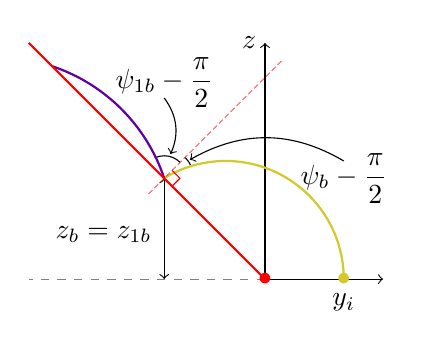
\begin{tikzpicture}[scale=1]
\draw[->] (0,0) to (0,3);


\node[] at (1,-0.3) {$y_i$};

\draw[-] (-1.28,1.28+0.286) arc (90:45:0.286);
\draw[-] (-1.28,1.28+0.286) arc (90:115:0.286);
\node at (-1.28,2.5) {$\psi_{1b}-\dfrac{\pi}{2}$};
\draw[->] (-1.28,2.3) to[bend left] (-1.2,1.28+0.306);


\draw[-] (-1.28+0.2652,1.28+0.2652) arc (45:22.5:0.375);

\node at (1,1.28) {$\psi_b - \dfrac{\pi}{2}$};
\draw[->] (1,1.5) to[bend right] (-1.28+0.3252,1.28+0.2352);


\draw[-,thick,black!20!yellow] (1,0) arc (0:180:1.5);
\draw[-,thick,purple!50!blue] (-1.28,1.28) arc (18.435:71.5653:2.25);

\draw[-,draw=none,fill=white] (-3,0) to (0,0) to (-3,3) to (-3,0);

\draw[<->] (-1.28,1.28) to (-1.28,0);
\node at (-2.05,0.57) {$z_b = z_{1b}$};

\draw[-,red,very thin,dashed,dash pattern=on 2pt off 1pt] (-1.28-0.2,1.28-0.2) to (-1.28+1.5,1.28+1.5);

\draw[-,dashed,black!50] (0,0) to (-3,0);
\draw[->] (0,0) to (1.5,0);

\node[red] at (0,0) {$\bullet$};
\node[black!20!yellow] at (1,0) {$\bullet$};

\draw[-,red,thick] (0,0) to (-3,3);


\draw[-,red] (-1.28+0.1,1.28+0.1) to (-1.28+0.2,1.28) to (-1.28+0.1,1.28-0.1);

\node at (-0.2,3) {$z$};
\end{tikzpicture}
\endpgfgraphicnamed
\end{document}

\section{Discussion}
\label{s:discussion}
\mySection{Related Works and Discussion}{}
\label{chap3:sec:discussion}

In this section we briefly discuss the similarities and differences of the model presented in this chapter, comparing it with some related work presented earlier (Chapter \ref{chap1:artifact-centric-bpm}). We will mention a few related studies and discuss directly; a more formal comparative study using qualitative and quantitative metrics should be the subject of future work.

Hull et al. \citeyearpar{hull2009facilitating} provide an interoperation framework in which, data are hosted on central infrastructures named \textit{artifact-centric hubs}. As in the work presented in this chapter, they propose mechanisms (including user views) for controlling access to these data. Compared to choreography-like approach as the one presented in this chapter, their settings has the advantage of providing a conceptual rendezvous point to exchange status information. The same purpose can be replicated in this chapter's approach by introducing a new type of agent called "\textit{monitor}", which will serve as a rendezvous point; the behaviour of the agents will therefore have to be slightly adapted to take into account the monitor and to preserve as much as possible the autonomy of agents.

Lohmann and Wolf \citeyearpar{lohmann2010artifact} abandon the concept of having a single artifact hub \cite{hull2009facilitating} and they introduce the idea of having several agents which operate on artifacts. Some of those artifacts are mobile; thus, the authors provide a systematic approach for modelling artifact location and its impact on the accessibility of actions using a Petri net. Even though we also manipulate mobile artifacts, we do not model artifact location; rather, our agents are equipped with capabilities that allow them to manipulate the artifacts appropriately (taking into account their location). Moreover, our approach considers that artifacts can not be remotely accessed, this increases the autonomy of agents.

The process design approach presented in this chapter, has some conceptual similarities with the concept of \textit{proclets} proposed by Wil M. P. van der Aalst et al. \citeyearpar{van2001proclets, van2009workflow}: they both split the process when designing it. In the model presented in this chapter, the process is split into execution scenarios and its specification consists in the diagramming of each of them. Proclets \cite{van2001proclets, van2009workflow} uses the concept of \textit{proclet-class} to model different levels of granularity and cardinality of processes. Additionally, proclets act like agents and are autonomous enough to decide how to interact with each other.

The model presented in this chapter uses an attributed grammar as its mathematical foundation. This is also the case of the AWGAG model by Badouel et al. \citeyearpar{badouel14, badouel2015active}. However, their model puts stress on modelling process data and users as first class citizens and it is designed for Adaptive Case Management.

To summarise, the proposed approach in this chapter allows the modelling and decentralized execution of administrative processes using autonomous agents. In it, process management is very simply done in two steps. The designer only needs to focus on modelling the artifacts in the form of task trees and the rest is easily deduced. Moreover, we propose a simple but powerful mechanism for securing data based on the notion of accreditation; this mechanism is perfectly composed with that of artifacts. The main strengths of our model are therefore : 
\begin{itemize}
	\item The simplicity of its syntax (process specification language), which moreover (well helped by the accreditation model), is suitable for administrative processes;
	\item The simplicity of its execution model; the latter is very close to the blockchain's execution model \cite{hull2017blockchain, mendling2018blockchains}. On condition of a formal study, the latter could possess the same qualities (fault tolerance, distributivity, security, peer autonomy, etc.) that emanate from the blockchain;
	\item Its formal character, which makes it verifiable using appropriate mathematical tools;
	\item The conformity of its execution model with the agent paradigm and service technology.
\end{itemize}
In view of all these benefits, we can say that the objectives set for this thesis have indeed been achieved. However, the proposed model is perfectible. For example, it can be modified to permit agents to respond incrementally to incoming requests as soon as any prefix of the extension of a bud is produced. This makes it possible to avoid the situation observed on figure \ref{chap3:fig:execution-figure-4} where the associated editor is informed of the evolution of the subtree resulting from $C$ only when this one is closed. All the criticisms we can make of the proposed model in particular, and of this thesis in general, have been introduced in the general conclusion (page \pageref{chap5:general-conclusion}) of this manuscript.





\subsection*{Acknowledgments}
We thank Patrick Flandrin, Adrien Hardy, and Fred Lavancier for fruitful
discussions on various aspects of this paper. RB acknowledges support from ANR
\textsc{BoB} (ANR-16-CE23-0003), and all authors acknowledge support from
ANR \textsc{BNPSI} (ANR-13-BS03-0006).
\bibliography{stft,stats}
\bibliographystyle{plainnat}

\end{document}
